% !TeX root = thesis.tex

% Vermijd bij dit hoofdstuk zeker kopieerwerk van bestaande documenten. Haal veeleer aan op welke manier de bouwblokken worden ingezet. Waar nodig refereren naar andere documenten of URL’s!

% Technologische bouwblokken. Overzicht van technologieën en methodologieën die relevant zijn voor de rest van je eindwerk. Begin met de helicopterview en zoom daarna in op de componenten die echt relevant zijn voor de rest van het eindwerk.

% Gerelateerd werk. Doe een scan van bestaand werk in je domein. Haal aan waar jouw oplossing verschilt t.o.v. bestaande oplossingen.

% Besluit.

 
\chapter{State of the art}\label{ch:sota}

\section{CCSDS}
The \gls{ccsds} is an international organisation of space agencies that formulate solutions for common problems in the development and operation of space data systems \cite{noauthor_ccsdsorg_nodate-1}. These solutions are called ''Recommended Standards''. % Nog meer uitleg want dees is maar mager 

The standards most related to this assignment are discussed below.

\subsection{CCSDS 121.0-b-3}
The \gls{ccsds} 121.0-b-3 recommended standard from august 2020 \cite{ccsds_secretariat_lossless_2020} is a lossless source coding data compression algorithm. It consists of two stages, the first stage being a preprocessor and the second stage an \gls{aec}.

The preprocessor's role is to convert the data by decorrelating and converting it into nonnegative integers with the preferred probability distribution. For the \gls{aec} a probability distribution approaching Laplacian is optimal. The preprocessor presented in this recommended standard is the \gls{unitdp}. This technique predicts the current sample using the one-sample delayed input data signal, this is illustrated in figure \ref{fig:udp}. 
\begin{figure}[h]
    \centering
    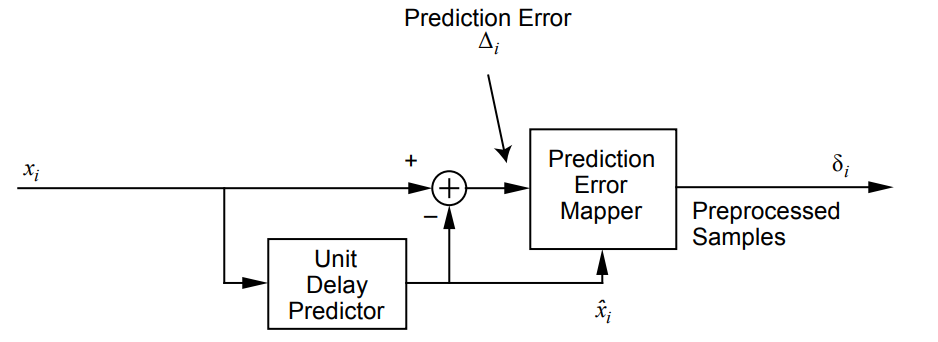
\includegraphics[width=0.7\textwidth]{figs/unit_delay_predictor.png}
    \caption{\acrfull{unitdp} \cite{ccsds_secretariat_lossless_2020}}
    \label{fig:udp}
\end{figure}


\subsection{CCSDS 122.0-b-2}
The \gls{ccsds} 1212.0-b-2 recommended standard from september 2017 \cite{ccsds_secreteriat_image_2017} is an image compression algorithm.

\subsection{Tests}


\section{FAPEC}
\subsection{Algorithm}
\gls{fapec} was developed by Portell, Villafranca and Garc\'{i}a-Berro \cite{portell_fapec_2018} as a way to overcome the problems of the CCSDS 121.0 Lossless Data Compression Recommendation. The idea behind \gls{fapec} was designing an algorithm that is capable of dealing with noise and outliers \cite{villafranca_fapec_2011}. It was made fully adaptive to automatically calibrate the algorithm to the statistics of the data, thus adapting to changes in the data distribution and becoming an completely autonomous coder.

The algorithm itself consists of a pre-processing (or decorrelation) stage followed by a coding stage \cite{portell_fapec_2018}. The pre-processing stage is oiften implemented by a data prediction algorithm or a transform such as the \gls{dwt}. In general this stage generates one output value for each input value. 
The \gls{fapec} core performs a statistical analysis on all individual prediction error blocks, identifying the morst effective coding tables and finally calling the \gls{pec} kernel, which produces a variable-length codefor each of the values to be coded. \gls{pec}

A more in-depth description of the algorithm can be found in \cite{portell_fapec_2018,villafranca_prediction_2013,villafranca_fapec_2011}.


\subsection{Tests}

\section{FELICS}
\subsection{Algorithm}
\gls{felics} is a technique presented by Paul G. Howard and Jeffrey Scott Vitter \cite{howard_fast_1993}.
\begin{figure}[h]
    \centering
    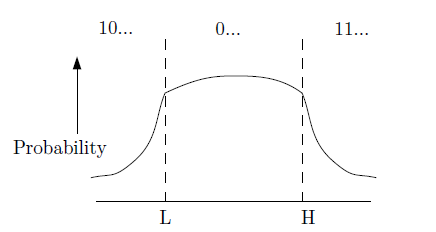
\includegraphics[width=0.5\textwidth]{figs/probability_intensity_P.png}
    \caption{Intensity distribution of new pixel \cite{howard_fast_1993}}
    \label{fig:dist}
\end{figure}
Each pixel is assigned a code depending on where its intensity (grey-scale value) is located relative to the intensities of its closest neighbours. The distribution of an image's intensity distribution is shown in figure \ref{fig:dist}. L denotes the smaller neighbouring intensity value, H denotes the larger neighbouring intensity value. There are three cases:
\begin{enumerate}
    \item The pixel's intensity P lies in the range [L, H]. One bit (0) is used to indicate the in-range position. Since the values of P are almost uniformly distributed, P is assigned an adjusted binary code that is slightly shorter at the centre of the region \cite{salomon_image_2010}.
    \item The pixel's intensity P is lower than L. Now, one bit (1) is used to indicate the out-of-range position, and one bit (0) is used to indicate the below-range position. 
    \item The pixel's intensity P is higher than H. Now, one bit (1) is used to indicate the out-of-range position, and one bit (1) is used to indicate the above-range position.  
\end{enumerate}

The probability of out-of-range values falls off sharply, making it reasonable to use exponential prefix codes like Golomb or Rice codes \cite{howard_fast_1993}.
A formal description of the algorithm can be found in \cite{howard_fast_1993}.

\subsection{Tests}


\section{mijn eigen ding}
\subsection{Algorithm}

\subsection{Tests}

\section{Hardware versus software-implementation}

\section{Conclusion}
% hierin korte samenvatting van de tests en zo vergelijking tussen de verschillende algoritmes maken
% NIETS NIEUWS VERTELLEN